%Chap 3 pag 51
\definecolor{DarkRed}{RGB}{128,0,0}
\definecolor{Green}{RGB}{0,100,0}

\begin{frame}{Búsqueda en profundidad}
Expandir el nodo no expandido más profundo.\\
\begin{center}
    \textit{\textcolor{Green}{franja}} = cola LIFO, es decir, poner sucesores al
    frente.\\
\end{center}{}

\textcolor{DarkRed}{Implementación:}
    \begin{figure}
        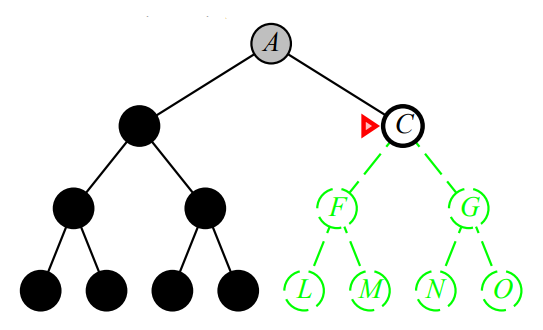
\includegraphics[scale=0.2]{51_chap3_pag51.png}
    \end{figure}
\end{frame}{}
